\documentclass[12pt,a4paper]{article}
\usepackage[ngerman]{babel}
\usepackage[utf8]{inputenc}
\usepackage[unicode=true,bookmarks=false,bookmarksopen=true]{hyperref}

\usepackage{xcolor}
\usepackage{graphicx}
\usepackage{tikz}

\usepackage{listings}

\def\checkmark{\tikz\fill[scale=0.4](0,.35) -- (.25,0) -- (1,.7) -- (.25,.15) -- cycle;}

\definecolor{pGreen}{rgb}{0.44, 0.71, 0}
\definecolor{nRed}{rgb}{0.74, 0, 0}

\title{ORES Custom Documentation V}
%\author{Tom Gülenman}
\date{}
\begin{document}
\maketitle
\textit{Disclaimer: No guarantee for the correctness of information / explanations / sources is given.}\\
%
\section*{Goals}
\begin{enumerate}
\item Metric list:
\begin{itemize}
\item Add examples \checkmark
\item Correct the descriptions of counts and rates \checkmark
\item Improve descriptions of roc\_auc and pr\_auc
\item Add the new standalone version to the repo
\end{itemize}
\item Research what form of revision data is needed (for existing visualizations, but also in general) $\rightarrow$ also check RecentChanges and new Filters and what API calls look like in that context
\item Watch \href{https://www.dataschool.io/roc-curves-and-auc-explained}{``ROC curves and Area Under the Curve explained''} and think about what parameters could be used in which ways to filter the output of the current UI (currently: X inputs $\rightarrow$ X outputs)
\begin{description}
\item Also check out: \href{https://www.kaggle.com/general/7517#post41179}{Precision-Recall AUC vs ROC AUC discussion}
\end{description}
\item Read \href{https://doi.org/10.1145/3185517}{A Review of User Interface Design for Interactive Machine Learning} (carefully!)
\item Think about what could be the goal of this thesis
\end{enumerate}
%
%
%
%TODO macro + micro
\newpage
\section{Crucial metrics: \textbf{damaging}-model}
Metrics simple list:\\

\begin{tabular}{| l | l |}
\hline 
!f1 & \checkmark \\ \hline
!precision & \checkmark \\ \hline
!recall & \checkmark \\ \hline
accuracy & \checkmark \\ \hline
counts & \checkmark \\ \hline
f1 & \checkmark \\ \hline
filter\_rate & \checkmark \\ \hline
fpr & \checkmark \\ \hline
match\_rate & \checkmark \\ \hline
pr\_auc & \checkmark \\ \hline 
precision & \checkmark\\ \hline
rates & \checkmark \\ \hline 
recall &  \checkmark\\ \hline
roc\_auc & \checkmark \\ \hline
\end{tabular}

\begin{description}
\item Again, changes have been made to the list and explanations, compared to the version in oresDoc4. The structure of explanations will be as follows:
\item For each metric (if possible) there will be:
\begin{enumerate}
\item The formula based on the \textbf{confusion matrix}
\item A definition
\item An intuitive explanation with an example
\item Its meaning based on the \textbf{loan threshold} representation by Google (\href{https://research.google.com/bigpicture/attacking-discrimination-in-ml/}{Link})
\item Additional information (if necessary)
\end{enumerate}
\end{description}
\subsection*{Explanations: References}
\begin{itemize}
\item Confusion Matrix 
\begin{description}
\item 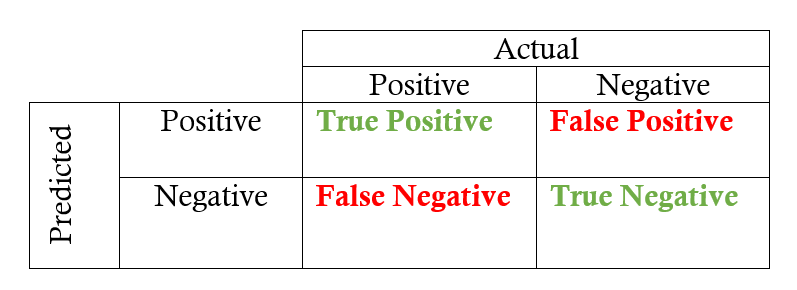
\includegraphics[scale=0.3]{resources/3/confusionMatrix}
\item Abbreviations: \textbf{\textcolor{pGreen}{TP}}, \textbf{\textcolor{nRed}{FP}}, \textbf{\textcolor{nRed}{FN}} and \textbf{\textcolor{pGreen}{TN}}.
\end{description}
\item Loan Threshold
\begin{description}
\item 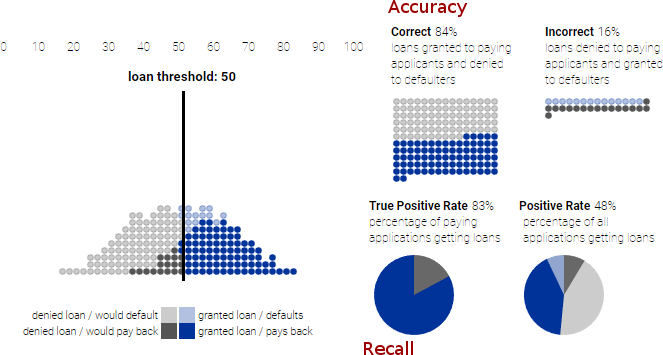
\includegraphics[scale=0.57]{resources/4/loanML4}
\end{description}
\end{itemize}
%
\subsection*{The example scenario}
To ease the understanding, let's stick to the following scenario and refer to it for each metric:
\begin{itemize}
\item 100 people represent our total population
\item 35\% of our population is infected with disease X
\begin{description}
\item That leaves us with the following \textbf{labels}: \textbf{35} \colorbox{pGreen}{\textbf{positives}} and \textbf{65} \colorbox{nRed}{\textbf{negatives}} (being tested for disease X;)
\item 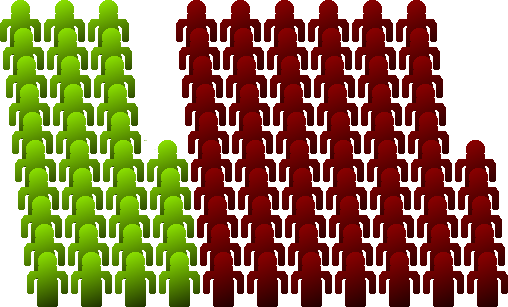
\includegraphics[scale=0.5]{resources/5/exampleBase}
\end{description}
\item A classifier is now supposed to classify every person of our population (based on their visible symptoms for example). This is the \textbf{prediction}:
\begin{itemize}
\item If our algorithm says a person is infected, that person will be classified as a \colorbox{pGreen}{\textbf{positive}}, and marked with radioactive symbol:
\begin{description}
\item 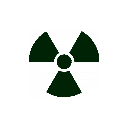
\includegraphics[scale=0.3]{resources/5/radioactive}
\end{description}
\item If the prediction results in a \colorbox{nRed}{\textbf{negative}}, the person will be marked with a sun symbol:
\begin{description}
\item 
\includegraphics[scale=0.3]{resources/5/sun}
\end{description}
\end{itemize}
\item The classifier may predict that:
\begin{itemize}
\item out of the 35 \colorbox{pGreen}{infected people}, \textbf{30} are infected (those 30 are what we call \textbf{true positives}) and \textbf{5} are not (those 5 are \textbf{false negatives}) 
\item out of the 65 \colorbox{nRed}{non infected people}, \textbf{10} are infected (\textbf{false positives}) and \textbf{55} are not (\textbf{true negatives})
\begin{description}
\item 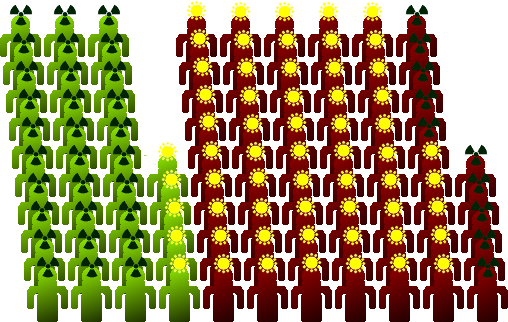
\includegraphics[scale=0.5]{resources/5/examplePredicted}
\item 
\includegraphics[scale=0.5]{resources/5/exampleTP} \textbf{true positive}: infected and correctly predicted (\textbf{30})
\item 
\includegraphics[scale=0.5]{resources/5/exampleFN} \textbf{false negative}: infected and incorrectly predicted (\textbf{5})
\item 
\includegraphics[scale=0.5]{resources/5/exampleTN} \textbf{true negative}: not infected and correctly predicted (\textbf{55})
\item 
\includegraphics[scale=0.5]{resources/5/exampleFP} \textbf{false positive}: not infected and incorrectly predicted (\textbf{10})
\end{description}
\end{itemize}
\end{itemize}

\paragraph{Let's get started.}
\subsection{recall}
\begin{enumerate}
\item $\frac{\texttt{TP}}{\texttt{TP} + \texttt{FN}}$
\item Recall ($\equiv$ true positive rate $\equiv$ ``sensitivity'') is the ability of a model to find \textbf{all} relevant cases within the dataset.
\item Now, in our example scenario, the relevant cases are the infected people. We absolutely want to identify those: 
\includegraphics[scale=0.3]{resources/5/exampleP}. The ability of the model to identify those depends on how many will be \textbf{correctly} predicted to be infected: 
\includegraphics[scale=0.3]{resources/5/exampleTP}.
\begin{description}
\item In other words, we are looking for the ratio of correctly predicted to be infected people to all infected people.
\item That leads to $\frac{\sum 
\includegraphics[scale=0.3]{resources/5/exampleTP}}{\sum 
\includegraphics[scale=0.3]{resources/5/exampleP}}$, with $
\includegraphics[scale=0.3]{resources/5/exampleP} = 
\includegraphics[scale=0.3]{resources/5/exampleTP} + 
\includegraphics[scale=0.3]{resources/5/exampleFN}$, which is equivalent to the formula in \textbf{1.}, if you replace the symbols with their confusion matrix counterpart according to the legend in \textbf{The example scenario}.
\item In terms of numbers for our example that would be $\frac{30}{30+5} \approx 0.86$
\end{description}
\item $\frac{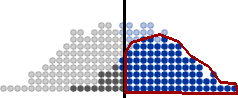
\includegraphics[scale=0.6]{resources/4/loanTP}}{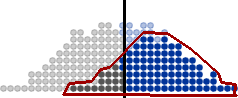
\includegraphics[scale=0.6]{resources/4/loanTP+FN}}$
\end{enumerate}
%
\subsection{precision}
\begin{enumerate}
\item $\frac{\texttt{TP}}{\texttt{TP} + \texttt{FP}}$
\item Ability of the model to find \textbf{only} relevant cases within the dataset
\item Again, we take a look at the relevant cases, the infected people: 
\includegraphics[scale=0.3]{resources/5/exampleP}. This time around though, we are \textbf{not} interested in the ratio of correctly predicted to be infected people to \textbf{all} infected people. Instead we want to know how good the model is at only predicting those to be infected, that actually are. Therefore, we want the ratio of all 
\includegraphics[scale=0.3]{resources/5/exampleTP} to all those predicted to be infected: $
\includegraphics[scale=0.3]{resources/5/exampleTP} + 
\includegraphics[scale=0.3]{resources/5/exampleFP}$
\begin{description}
\item $= \frac{\sum 
\includegraphics[scale=0.3]{resources/5/exampleTP}}{\sum 
\includegraphics[scale=0.3]{resources/5/exampleTP} + \sum 
\includegraphics[scale=0.3]{resources/5/exampleFP}} = \frac{30}{30+10} = 0.75$
\end{description}
\item $\frac{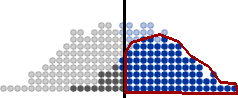
\includegraphics[scale=0.6]{resources/4/loanTP}}{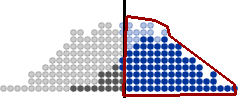
\includegraphics[scale=0.6]{resources/4/loanTP+FP}}$
\end{enumerate}
%
\subsection{f1}
\begin{enumerate}
\item -
\item f1-Score, the harmonic mean of recall and precision, a metric from \textbf{0} (worst) to \textbf{1} (best), used to evaluate the accuracy of a model by taking into account recall and precision: $=2*\frac{\texttt{precision} * \texttt{recall}}{\texttt{precision}+\texttt{recall}}$
\item For our example model, that would result in $=2*\frac{0.75 * \frac{30}{35}}{0.75+\frac{30}{35}} = 0.8$
\item -
\item \underline{Additional information}: Compared to the simple average (of recall and precision), the harmonic mean punishes extreme values (e.g. precision 1.0 and recall 0.0 $\rightarrow$ average = 0.5, but f1 $= 0$)
\end{enumerate}
%
\subsection{fpr}
\begin{enumerate}
\item $\frac{\texttt{FP}}{\texttt{FP} + \texttt{TN}}$
\item The false positive rate is the probability of a false alarm.
\item In our example, a false alarm would obviously be labeling someone as infected, who isn't: 
\includegraphics[scale=0.3]{resources/5/exampleFP}. Now we just have to ask ourselves what portion of those, that, if they \textbf{were} incorrectly predicted as infected (because they \textbf{are not} infected: 
\includegraphics[scale=0.3]{resources/5/exampleN}), \textbf{are} incorrectly predicted as infected? Hence, we are looking for the ratio of 
\includegraphics[scale=0.3]{resources/5/exampleFP} to all non infected people: $
\includegraphics[scale=0.3]{resources/5/exampleFP} + 
\includegraphics[scale=0.3]{resources/5/exampleTN}$.
\begin{description}
\item $= \frac{\sum 
\includegraphics[scale=0.3]{resources/5/exampleFP}}{\sum 
\includegraphics[scale=0.3]{resources/5/exampleFP} + \sum 
\includegraphics[scale=0.3]{resources/5/exampleTN}} = \frac{10}{10+55} \approx 0.15$
\end{description}
\item $\frac{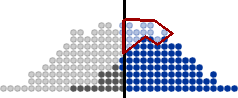
\includegraphics[scale=0.6]{resources/4/loanFP}}{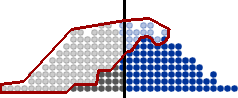
\includegraphics[scale=0.6]{resources/4/loanTN+FP}}$
\end{enumerate}
\subsection{roc\_auc}
\begin{enumerate}
\item -
\item The \textbf{area under} the \textbf{curve} of the \textbf{ROC}-curve, a measure between 0.5 (worthless) and 1.0 (perfect: getting no FPs), rates the ability of a model to achieve a blend of recall and precision.
\item In our example, we haven't used the notion of threshold yet. For classifying people as infected or not, the classifier will evaluate multiple criteria and calculate the probability that a patient is infected. Many binary classifiers have the threshold at 0.5, meaning that, if the probability of a true outcome is higher than 50\%, it is classified as a positive; or in our case as an infected patient. Depending on the situation however, it can be useful to move that threshold.
\begin{description}
\item  The receiver operating characteristic (ROC) curve is used to visualize the performance of a classifier
\item The ROC curve plots the TPR versus FPR as a function of the model’s threshold for classifying a positive.
\item 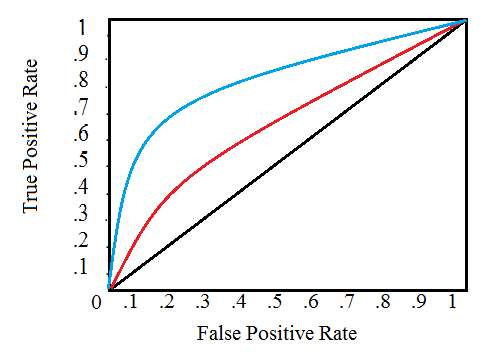
\includegraphics[scale=0.5]{resources/3/ROCcurve}
\item Increasing the threshold $\rightarrow$ moving up a curve ($\equiv$ model) to the top right corner, where all data is predicted as positive (threshold = 1.0) and vice versa
\item Our best case is a curve hugging the top left corner, because that means a low \textbf{fpr} and high \textbf{tpr}, which, again, means a lot of positives and few negatives on the right of the thresholds, looking at class curves like the \textbf{Loan Threshold} one.
\item Assuming that we have had a threshold of 0.5 all along to get the previous results, one point on our ROC curve would be: $(0.15,0.86)=(\texttt{fpr},\texttt{tpr})$.
\item We would now have to change the thresholds, look at the (probably) changed resulting data (new numbers in terms of positives and negatives, as well as \textbf{TP}, \textbf{FN}, \textbf{TN} and \textbf{FP}) and then plot every resulting $(\texttt{fpr},\texttt{tpr})$-point in order to plot the full ROC curve.
\item We would most certainly like to quantify this visualized performance of our binary classifier, which is why we calculate the area under the curve (\textbf{auc}) of the ROC curve.
\end{description}
\item -
\item \underline{Additional information}: We can think of AUC as representing the probability that a classifier will rank a randomly chosen positive observation higher than a randomly chosen negative observation. That's why \textbf{roc\_auc} is a useful metric even for datasets with highly unbalanced classes. (\href{https://www.youtube.com/watch?v=OAl6eAyP-yo}{Source})
\end{enumerate}
%
\subsection{pr\_auc}
\begin{enumerate}
\item -
\item Similarly to the \textbf{roc\_auc}, the area under the precision recall curve \textbf{pr\_auc} evaluates a classifiers performance. The main difference, however, is that the \textbf{pr\_auc} does not make use of \textbf{true negatives}. It is therefore favourable to use \textbf{pr\_auc} over \textbf{roc\_auc} if true negatives are unimportant to the general problem or if there are a lot more negatives than positives.
\begin{description}
\item The PR-curve plots the Precision versus the Recall:
\item 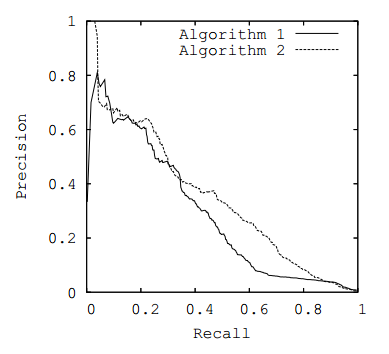
\includegraphics[scale=0.7]{resources/3/PRcurve}
\item Instead of the top left corner for the ROC-curve, here, we want our curve to reach the top right corner for our classifier to be perfect.
\end{description}
\begin{description}
\item The following scenario provides a good example (\href{https://www.kaggle.com/general/7517#post41179}{Source 1} and \href{http://www.chioka.in/differences-between-roc-auc-and-pr-auc/}{Source 2}) of a case with a lot more negatives than positives and comparing ROC to PR:
\begin{itemize}
\item Out of 1 million documents, we want to find the 100 relevant ones.
\item The task is accomplished by two different algorithms:
\begin{enumerate}
\item 100 retrieved documents, 90 relevant
\item 2000 retrieved documents, 90 relevant
\end{enumerate}
\item Algorithm (a) is obviously preferable.
\item We know that ROC- and PR-curves both plot coordinates with $\texttt{tpr} = \texttt{recall}$ as one dimension. Now the question is: how do they differ in the other dimension, when plotting both algorithms?
\item In all cases $\texttt{tpr} = \texttt{recall} = 0.9$. We also have:
\begin{enumerate}
\item $\texttt{TN} = 999890$ and $\texttt{FP} = 10$
\item $\texttt{TN} = 997990$ and $\texttt{FP} = 1910$
\end{enumerate}
\item \colorbox{yellow}{ROC}:
\begin{enumerate}
\item $\texttt{fpr}= \frac{\texttt{FP}}{\texttt{FP+TN}} = \frac{10}{10+999890} = 0.00001$
\item $\texttt{fpr}= \frac{1910}{1910+997990} = 0.00191$
\begin{description}
\item Having retrieved many more documents, and therefore having many more \textbf{false positives}, algorithm (b) has a higher \textbf{fpr} than algorithm (a). 
\item The \textbf{fpr} also takes into account the vast amount of \textbf{true negatives} though, which is why the difference between the two \textbf{fpr}s is still quite small: $0.0019$.
\end{description}
\end{enumerate}
\item \colorbox{yellow}{PR}:
\begin{enumerate}
\item $\texttt{precision}= \frac{\texttt{TP}}{\texttt{TP+FP}} = \frac{90}{90+10} = 0.9$
\item $\texttt{precision}= \frac{90}{90+1910} = 0.045$
\begin{description}
\item Not accounting for \textbf{true negatives}, the \textbf{precision} is not affected by the relative imbalance.
\item We are presented a remarkable difference of $0.855$.
\end{description}
\end{enumerate}
\item To close on this topic, not the following (by Randy C): ``Obviously, those are just single points in ROC and PR space, but if these differences persist across various scoring thresholds, using ROC AUC, we'd see a very small difference between the two algorithms, whereas PR AUC would show quite a large difference.''
\end{itemize}
\end{description}  
%
\item Similarly to the \textbf{roc\_auc}, the point on the PR curve of our example for the standard threshold of 0.5 would be: $(\texttt{precision},\texttt{recall}) = (0.75.0.86)$.
\item -
\end{enumerate}
%
\subsection{accuracy}
\begin{enumerate}
\item $\frac{\texttt{TP}+\texttt{TN}}{\texttt{Total}}$
\item Accuracy measures the portion of correctly predicted data
\item In our example scenario, this is equal to asking ourselves \textit{out of all patients, what's the portion of correctly predicted cases?} The correctly predicted cases are infected patients, predicted to be infected ( 
\includegraphics[scale=0.3]{resources/5/exampleTP} ), and non infected patients, predicted not to be infected ( 
\includegraphics[scale=0.3]{resources/5/exampleTN} ). This wanted proportion results in: 
\begin{description}
\item $= \frac{\sum 
\includegraphics[scale=0.3]{resources/5/exampleTP} + \sum 
\includegraphics[scale=0.3]{resources/5/exampleTN}}{\sum 
\includegraphics[scale=0.3]{resources/5/exampleP} + \sum 
\includegraphics[scale=0.3]{resources/5/exampleN}} = \frac{30+55}{35+65} = 0.85$
\end{description}
\item $\frac{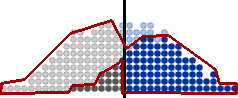
\includegraphics[scale=0.6]{resources/4/loanTP+TN}}{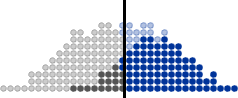
\includegraphics[scale=0.6]{resources/4/loanTotal2}}$
\end{enumerate}
\subsection{match\_rate}
\begin{enumerate}
\item $\frac{\texttt{TP}+\texttt{FP}}{\texttt{Total}}$
\item The match rate is the proportion of observations matched/not-matched, meaning the ratio of observations predicted to be positive to the total of observations.
\item Concerning our example, this would be equal to wanting to know what portion of the population was predicted to be infected. Those groups are: 
\includegraphics[scale=0.3]{resources/5/exampleTP} and 
\includegraphics[scale=0.3]{resources/5/exampleFP}.
\begin{description}
\item \item $= \frac{\sum \includegraphics[scale=0.3]{resources/5/exampleTP} + \sum \includegraphics[scale=0.3]{resources/5/exampleFP}}{\sum \includegraphics[scale=0.3]{resources/5/exampleP} + \sum \includegraphics[scale=0.3]{resources/5/exampleN}} = \frac{30+10}{35+65} = 0.4$
\end{description}
\item $\frac{\includegraphics[scale=0.6]{resources/4/loanTP+FP}}{\includegraphics[scale=0.6]{resources/4/loanTotal2}}$
\end{enumerate}
%
\subsection{filter\_rate}
\begin{enumerate}
\item $1-\texttt{match\_rate} = \frac{\texttt{TN}+\texttt{FN}}{\texttt{Total}}$
\item The filter rate is the proportion of observations filtered/not-filtered, meaning the ratio of observations predicted to be negative to the total of observations. This is the complement to the match rate.
\item In our example scenario, this would be equal to wanting to know what portion of the population was predicted not to be infected.
\begin{description}
\item $= \frac{\sum \includegraphics[scale=0.3]{resources/5/exampleTN} + \sum \includegraphics[scale=0.3]{resources/5/exampleFN}}{\sum \includegraphics[scale=0.3]{resources/5/exampleP} + \sum \includegraphics[scale=0.3]{resources/5/exampleN}} = \frac{55+5}{35+65} = 0.6 = 1- \texttt{match\_rate}$
\end{description}
\item $\frac{\includegraphics[scale=0.6]{resources/4/loanTN+FN}}{\includegraphics[scale=0.6]{resources/4/loanTotal}}$
\end{enumerate}
%
\subsection{counts}
\begin{enumerate}
\item \begin{itemize}
\item \textbf{labels}:
\begin{itemize}
\item false:  $\texttt{TN}+\texttt{FP}$
\item true: $\texttt{TP}+\texttt{FN}$
\end{itemize}
\item \textbf{n}: $\texttt{Total}$
\item \textbf{predictions}:
\begin{itemize}
\item false:
\begin{itemize}
\item false: $\texttt{TN}$
\item true: $\texttt{FP}$
\end{itemize}
\item true:
\begin{itemize}
\item false: $\texttt{FN}$
\item true: $\texttt{TP}$
\end{itemize}
\end{itemize}
\end{itemize}
\item \begin{itemize}
\item \textbf{labels}: The number of edits (\textit{manually}) labeled as \textit{false} and \textit{true}: these values represent the \textbf{actual} positives and negatives.
\item \textbf{n}: The sample size; total number of edits taken into account
\item \textbf{predictions}: \textcolor{blue}{edits ...}
\begin{itemize}
\item false: \textcolor{nRed}{... actually being false ...}
\begin{itemize}
\item false: \textcolor{nRed}{... and predicted to be false}
\item true: \textcolor{nRed}{... but predicted to be true}
\end{itemize}
\item true: \textcolor{pGreen}{... actually being true ...}
\begin{itemize}
\item false: \textcolor{pGreen}{... but predicted to be false}
\item true: \textcolor{pGreen}{... and predicted to be true}
\end{itemize}
\end{itemize}
\end{itemize}
\item Concerning our example:
\begin{itemize}
\item \textbf{labels}:
\begin{itemize}
\item false (\textcolor{nRed}{non infected people}): $\includegraphics[scale=0.3]{resources/5/exampleTN}+\includegraphics[scale=0.3]{resources/5/exampleFP}=55+10=65$ 
\item true (\textcolor{pGreen}{infected people}): $\includegraphics[scale=0.3]{resources/5/exampleTP}+\includegraphics[scale=0.3]{resources/5/exampleFN}= 30+5=35$
\end{itemize}
\item \textbf{n} (Total): $100$
\item \textbf{predictions}:
\begin{itemize}
\item false (\textcolor{nRed}{non infected people ...})
\begin{itemize}
\item false (\textcolor{nRed}{... and predicted not to be infected}): $\includegraphics[scale=0.3]{resources/5/exampleTN} = 55$
\item true (\textcolor{nRed}{... but predicted to be infected}): $\includegraphics[scale=0.3]{resources/5/exampleFP} = 10$
\end{itemize}
\item true (\textcolor{pGreen}{infected people ...})
\begin{itemize}
\item false (\textcolor{pGreen}{... predicted not to be infected}): $\includegraphics[scale=0.3]{resources/5/exampleFN} = 5$
\item true (\textcolor{pGreen}{... predicted to be infected}): $\includegraphics[scale=0.3]{resources/5/exampleTP} = 30$
\end{itemize}
\end{itemize}
\end{itemize}
\item -
\item \underline{Additional information}:
\begin{description}
\item When calling the enwiki damaging model for example (\href{https://ores.wikimedia.org/v3/scores/enwiki/?models=damaging&model_info=statistics}{Link}), you will get the following output for counts:
\item \includegraphics[scale=0.7]{resources/4/enwikiDamagingCounts}
\item $\Rightarrow$ e.g. out of 18677 edits that were labeled as \textit{false}, 719 were false positives
\end{description}
\end{enumerate}
%
\subsection{rates}
\begin{enumerate}
\item \begin{itemize}
\item false: $\frac{\texttt{counts\_labels\_false}}{\texttt{counts\_n}}$
\item true: $\frac{\texttt{counts\_labels\_true}}{\texttt{counts\_n}}$
\end{itemize}
\item The rates simply give us the proportion of edits labeled as false or true to the total number of edits taken into account.
\item For the example scenario: 
\begin{itemize}
\item false (proportion of infected people to the total number of people tested): $\frac{\sum \includegraphics[scale=0.3]{resources/5/exampleN}}{100} = \frac{65}{100} = 0.65$
\item true (proportion of infected people to the total number of people tested): $\frac{\sum \includegraphics[scale=0.3]{resources/5/exampleP}}{100} = \frac{35}{100} = 0.35$
\end{itemize}
\item -
\item \underline{Additional information}:
\begin{description}
\item Calling the API the same way as for \textbf{counts} (\href{https://ores.wikimedia.org/v3/scores/enwiki/?models=damaging&model_info=statistics}{Link}), we get:
\item \includegraphics[scale=0.7]{resources/4/enwikiDamagingRates}
\item The number of edits taken into account for \textbf{sample} equals the \textbf{n} from \textbf{counts} $= 19428$.
\item Now we see that, also looking at the output under \textbf{counts}, \textit{rates\_sample\_false}: $0.961 = \frac{18677}{19428}$.
\item Note that we are shown results for ``population'' and ``sample''. There is a significant number of bot edits and edits that don't need reviewing (admins, autopatrolled users). The \textbf{sample} of edits does not contain any of those.
\end{description}
\end{enumerate}

%
%TODO change anything here?
\subsection{!$<$metric$>$}
\begin{itemize}
\item Any $<$metric$>$ with an exclamation mark is the same metric for the negative class
\item e.g. recall $= \frac{\texttt{TP}}{\texttt{TP} + \texttt{FN}} \Rightarrow$ \textbf{!}recall  $= \frac{\texttt{TN}}{\texttt{TN} + \texttt{FP}}$
\item Example usage: find all items that are not ``E'' class $\rightarrow$ look at \textbf{!}recall for ``E'' class.
\end{itemize}
\subsubsection{Existing !$<$metric$>$s}
\begin{itemize}
\item !f1
\item !precision
\item !recall
\end{itemize}
%
\subsection{Additional explanations}
\subsubsection{recall vs precision}
When increasing one of these two, the other one naturally decreases. For an intuitive example, let's take a look at \href{https://research.google.com/bigpicture/attacking-discrimination-in-ml/}{Google's Loan Threshold Simulation}:\\
\includegraphics[scale=0.6]{resources/3/loanML3}\\
\begin{description}
\item The dark grey / dark blue dots, representing clients that would actually pay back their loan, are more and more included ($\rightarrow$ given loans) if we move the threshold further to the left.
\item But so are clients that would not. Thus moving the threshold to the left increases the \textbf{recall} (\textbf{tpr}) but decreases the \textbf{precision} and vice versa when moving to the right.
\end{description}
%
\subsubsection{roc\_auc vs pr\_auc}
see: \url{https://www.kaggle.com/general/7517}
\begin{itemize}
\item tl;dr: if the class imbalance problem exists, \textbf{pr\_auc} is more appropriate than \textbf{roc\_auc}
\begin{description}
\item If TNs are not meaningful to the problem or there are a lot more negatives than positives, \textbf{pr\_auc} is the way to go (it does not account for TNs).
\end{description}
\item In other words: 
\begin{itemize}
\item If the model needs to perform equally on the positive and negative class $\rightarrow$ \textbf{roc\_auc}
\item If it's not interesting how the model performs on negative class $\rightarrow$ \textbf{pr\_auc} (example: detecting cancer; find all positives and make sure they're correct!)
\end{itemize}
\end{itemize}
%
%
%
%
\section*{Questions}
\begin{itemize}
%
\item \colorbox{yellow}{Q:} Should I ask Aaron how he would like us to work together? I'm not sure how he meant it.
\begin{description}
\item \colorbox{orange}{A:} 
\end{description}
%
\item \colorbox{yellow}{Q:} In what situations exactly do we want to optimize the threshold in the context of user centered threshold optimization?
\begin{description}
\item \colorbox{orange}{A:} 
\end{description}
%
\end{itemize}
\end{document}